\section{Design Motivation}
\textit{Crossfire} has three main design goals: multiprocess support, remote and
mobile debug, and open Web, cross-browser debugging.
These closely related goals arose out of an interplay between user benefit and development costs.
As an open source project we must work with development resources motivated by
goals: no matter how much value Firebug users may recieve from a goal, the
selection must be limited by the motivation of open source contributors.

Necessity motivated first \textit{Crossfire} design goal, multiprocess support.
Soon after the Google Chrome browser was released, the Firefox team at Mozilla
began plans to convert Firefox to a multi-processor design.  The Google browser
used one controlling process for the application and one process for each Web
page.  This allows the browser to use the operating system isolation to prevent
problems on one page from bringing down the entire application and it allows
each page to use a different physical processor on modern multi-core computers
\cite{GoogleChrome}.  Depending upon the Firefox browser plaform changes, a
shift to multiprocess could render Firebug unusable. As a practical matter we
could not wait to for the new platform to be available: with only two full-time
developers plus a number of dedicated but part time contributors, and a commitment to continous
compatibility with Firefox we had to begin work immediately to insure that our
small resource could complete the transition in time to remain a viable project.
Therefore we assumed that Firefox would adopt an architecture similar to Google
Chrome: a client/server split debugger with a backend in one Web page process
and a front end in another process.  We believe that this assumption is planning
for the worst case: converting Firebug to client/server is a multi-person-year
effort but very likely to work with what ever the Firefox team decides to do.

While necessity forced our action, opportunity followed. The client/server
choice, if successful, adds two new dimensions to Firebug for users: remote
debug and mobile device debug. We expect the value of these dimensions to grow
as more developers work in distributed teams and as mobile plays an increasingly
important role in Web application development.  In fact this value was
recognized by the DragonFly Web debugger for Opera well before even the Google
Chrome browser.   The additional cost of designing for remote and mobile debug
on top of a client/server design -- primarily mechanisms for specifying the
connection addresses -- comes with high potential benefit.  Moreover, the benefit
aligns with directions important to the project's primary open source
contributors (one full time person from IBM and Mozilla).

The final goal, open Web, cross-browser debugging, offers even more benefits to
Firebug users.  Web application developers by definition target all Web users,
but all Web users are not running identical Web platforms. Almost all
potential users of a Web site will be running one of few similar but slightly
different browsers. The commonality allows Web developers to do most of their
work on one browser, then test for differences on other browsers. Of course in
the latter case they need to debug the problem on a browser with unfamilar debugging
tools. A common debugging tool across the major browsers would help with this
common and significant problem.

The benefit of cross-browser debugging comes at a steep cost for the project.
Instead of one server and one client, we face at minimum one server for every
browser. And for each server we have to deal with both the slight differences in
browser implementation of standard Web APIs and potential large differences in
how debuggers can connect to the browser.

Unlike commerical or pure research projects, an open source project like Firebug
might balance the cost of
implementing cross-browser debugging support by attracting more contributors
interested in this particular goal. That is, by adding this costly goal we can
attract new contributors, allowing us to create more total value. In particular
new contributors from the Orion project\cite{orion}, joined to create
\textit{Crossfire} server for Microsoft Internet Explorer and from the Eclipse
project\cite{EclipseJSDT} to create new \textit{Crossfire} client in Java for
connecting to Eclipse.   Moreover, a cross-browser client for Web debugging can be largely
implemented with Firebug Lite code, allowing our project to consolidate
developer resources around fewer lines of code to maintain.

Our three design goals created constraints for the \textit{Crossfire} implementation.
Above we outlined
how the multiprocess support lead to a client-server design choice. Support for
remote and mobile debug forces isolation of user interface to the client
(excepting some small interface for connection specification). The cross-browser
goal creates constraints indirectly: to minimize the extra cost of supporting
multiple servers we chose to adopt the Google Chrome communications channel
(sockets) and wire protocol format (JSON). Neither Firefox nor Internet Explorer
had existing servers, so they did not alter our choices. Opera had a server but
no one on our open source team planned to work with Opera and the server itself
was not open source making implementation more difficult.  Since Firebug is
already written in JavaScript, JSON format is especially easy to work with and
has good performance\cite{JSON}.  For the communications protocol, HTTP would be
a better choice for the project: the JavaScript support for HTTP is much better
than sockets and HTTP works better in practical remote scenarios through
firewalls.  However we made the judgement that better socket support was coming
in future\cite{WebSockets}, support was adequate now, and lowering cost on the
Google Chrome server was important.  In addition our goals imply that the
client and the communication protocol should be built from open web standards to
maximize the reuse across servers.

\section{Evolution not Revolution}
In addition to motivating developers to contribute to \textit{Crossfire}, we also need to motivate users
to help us test and refine the system.
As a practical project supporting 3 million users, Firebug
provides a large base of experienced Web developers working with a broad spectrum of Web technologies.
An open source, working, state-of-the-art debugger motivates users to explain problems, create test cases,
provide documentation and to help other users with problems that come up. To harness this
 unusual resource  for \textit{Crossfire} we need a plan for incremental refactoring of Firebug to be compatible
with \textit{Crossfire}.  The refactoring plan needs to provide waypoints for the development and it needs to
provide intermediate value to users and/or contributors.

\subsection{Inter-application JavaScript Debugging}
The first intemediate state for \textit{Crossfire} is shown in Fig.\ref{fig:fireclipse}.
\begin{figure}[htp]
  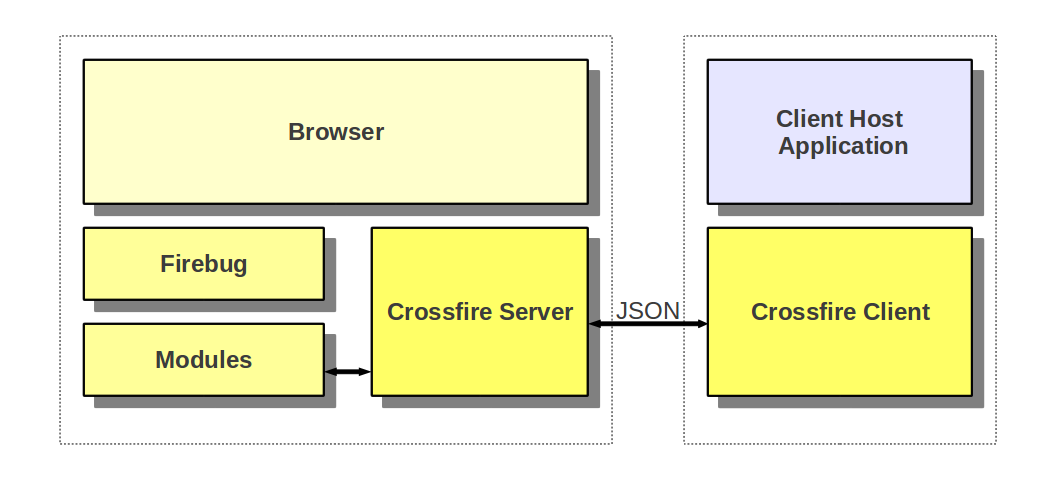
\includegraphics  [width = 86 mm] {figures/fireclipse.png}
  \caption{Inter-application JavaScript Debugging \textit{Crossfire} architecture.
\textit{Crossfire} versions 0.1 to 0.3 connected to an Eclipse plugin, supporting simple JavaScript debugging}
 \label{fig:fireclipse}
\end{figure}
In Firefox we implemented a \textit{Crossfire} server limited to support for JavaScript debugging.
In Eclipse we implemented a \textit{Crossfire} client. This allows the user interface in Eclipse to control
 and examine the JavaScript program running
in Firefox.  A closed-source version of the client shipped in IBM's Rational Application Developer product for two years,
then the open source Eclipse team created a new implementation as part of it's JavaScript Developer
Tools (JSDT) project\cite{JSDT}.  By working towards the Eclipse team goals of
remote JavaScript debugging, this stage of the work provided valuable implementation 
experience and engagement with the Eclipse team.
This work is largely complete.

\subsection{Intra-browser JavaScript Debugging}
The second intermediate state implements the client side of the JavaScript part of \textit{Crossfire} in
a Web browser as sketched in Fig.~\ref{fig:fbugChrome}.
\begin{figure}[htp]
  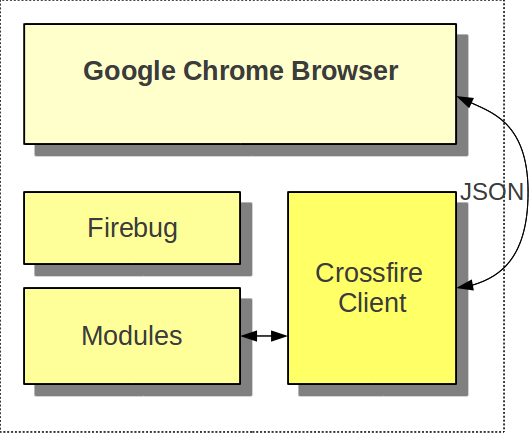
\includegraphics  [width = 86 mm] {figures/fbugChrome.png}
  \caption{Intra-browser JavaScript Debugging \textit{Crossfire} architecture.
\textit{Crossfire} versions 0.4 targets supporting simple JavaScript debugging with the client and server in the same application.}
 \label{fig:fbugChrome}
\end{figure}
While this diagram seems a bit bizarre, with the
debugger running in and connecting back into the the same browser, this step allows us to add JavaScript debug
support to the Firebug Lite implementation in the Google Chrome browser while we simultaneuously refactor
the Firefox  \textit{Crossfire} server to resemble the Google Chrome back end.

The key reason this architecture makes sense is that a large part of the non-JavaScript parts of a Web page
debugger uses standard Web APIs. That  means that three different applications, Firebug Lite running as co-resident with a Web page,
Firebug Lite running as a Google Chrome extension,  and the HTML/CSS/Console debug support code in Firebug
for Firefox can use identical code in different wrappers. By re-engineering our current somewhat divergent code
to group the idential parts we reduce maintainence. By adding for JavaScript debugging using the newly platform-independent Firefox code to the Firebug for Google Chrome code we add user value: the beginnings of cross browser development. Both efforts contribute to our final goals.

Furthermore, the two JavaScript-only \textit{Crossfire} servers, one for Firefox and one for Google Chrome, can support
alternative clients. In particular, the Orion project, a Web based Web-development system, plans to support
JavaScript debugging over \textit{Crossfire} on their editor user interface. In
return that project is implementing a \textit{Crossfire} server for Internet Explorer, allowing us to cover more than 75\% of the browser market with \textit{Crossfire} supported tools.
This work is scheduled to complete in June, 2011.

\subsection{Cross-browser Debugging}
The final stage completes the tranformation of an in-process single browser Web
page debugger to a client-server cross-browser tool as shown in
Fig.~\ref{fig:crossbrowser}. \begin{figure}[htp]
  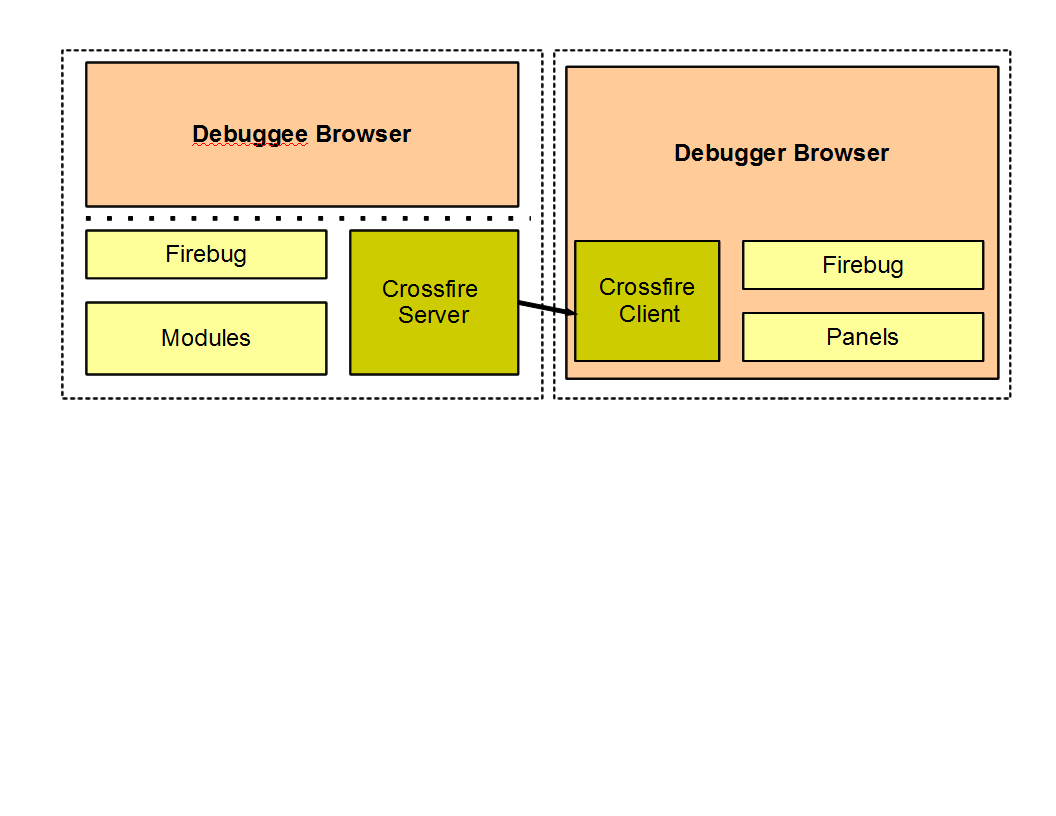
\includegraphics  [width = 86 mm] {figures/crossbrowser.png}
  \caption{Cross-browser Debugging architecture, proposed.}
 \label{fig:crossbrowser}
\end{figure}
Conceptually we simply re-apply the approach ironed out in the previous step to
the rest of the program and arrive at the complete value proposed at the outset.
In practice, the concept hides a lot of work. Lots of lines of code must be
carefully divide into two piles and the whole must get working again. This work
is scheduled to complete in Dec. 2011.
